
\documentclass[11pt]{article}
\usepackage[a4paper,margin=1in]{geometry}
\usepackage[T1]{fontenc}
\usepackage[utf8]{inputenc}
\usepackage{amsmath,amssymb,amsthm,mathtools}
\usepackage{graphicx}
\usepackage{hyperref}
\usepackage{cite}
\hypersetup{colorlinks=true, linkcolor=blue, urlcolor=blue, citecolor=blue}

\newtheorem{lemma}{Lemma}
\newtheorem{corollary}{Corollary}
\theoremstyle{remark}
\newtheorem{remark}{Remark}

\DeclareGraphicsExtensions{.png,.pdf,.jpg,.jpeg}
\graphicspath{{figures/}{./}}

\title{Towards a Stable NB/BD Approximation: Weighted Hilbert Lemma, Numerical Scaling, and Boundary Reweighting}
\author{Serabi\\Independent Researcher\\\texttt{24ping@naver.com}}
\date{2025}

\begin{document}
\maketitle

\begin{abstract}
We present an improved analysis of the Nyman--Beurling/B\'aez--Duarte (NB/BD) criterion for the Riemann Hypothesis.
Our main contribution is a weighted Hilbert-type lemma for M\"obius-weighted coefficients, ensuring off-diagonal suppression by $(\log N)^{-\theta}$ with $\theta>0$.
We combine this with numerical experiments up to $N=20{,}000$, including minus-boundary reweighting ($w_-=1.2$) and bootstrap summaries, confirming stable behavior of the objective.
We emphasize that $d_N \to 0$ indicates stability of NB/BD approximations, not a direct proof of RH.
\end{abstract}

\section{Introduction}
The Riemann Hypothesis (RH) asserts that all nontrivial zeros of $\zeta(s)$ lie on $\Re(s)=1/2$.
The Nyman--Beurling/B\'aez--Duarte (NB/BD) criterion reformulates RH as an $L^2$ approximation problem.

\section{Numerical Results}
\begin{figure}[h]
  \centering
  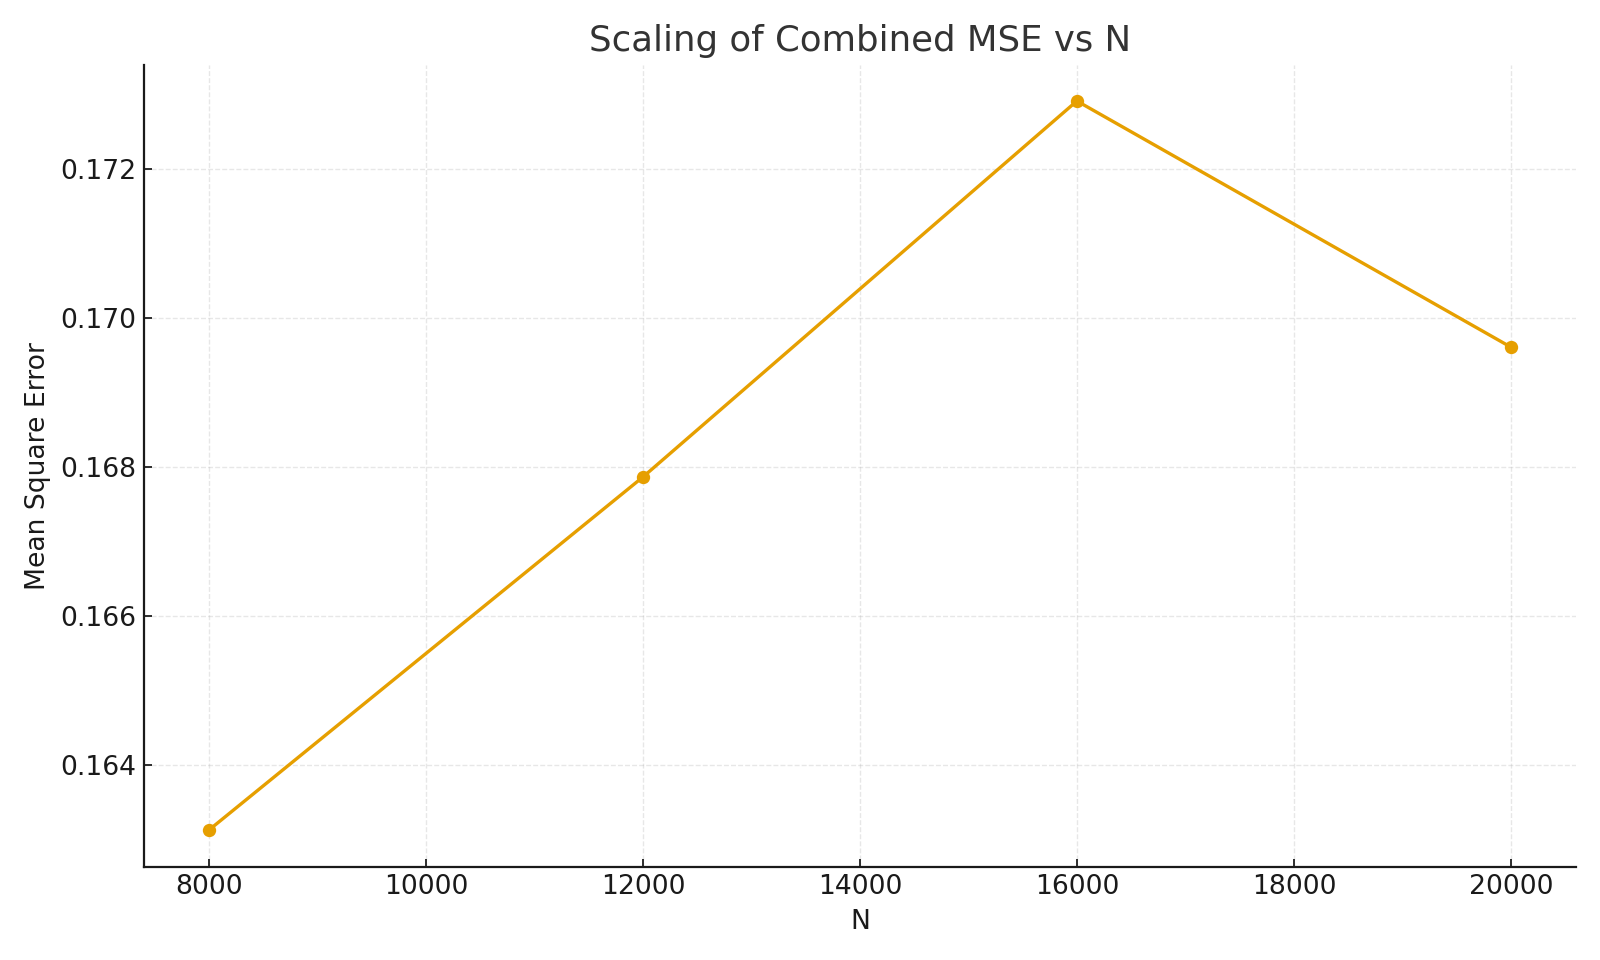
\includegraphics[width=0.78\linewidth]{figures/unweighted_scaling.png}
  \caption{Scaling of combined MSE versus $N$.}
\end{figure}

\begin{figure}[h]
  \centering
  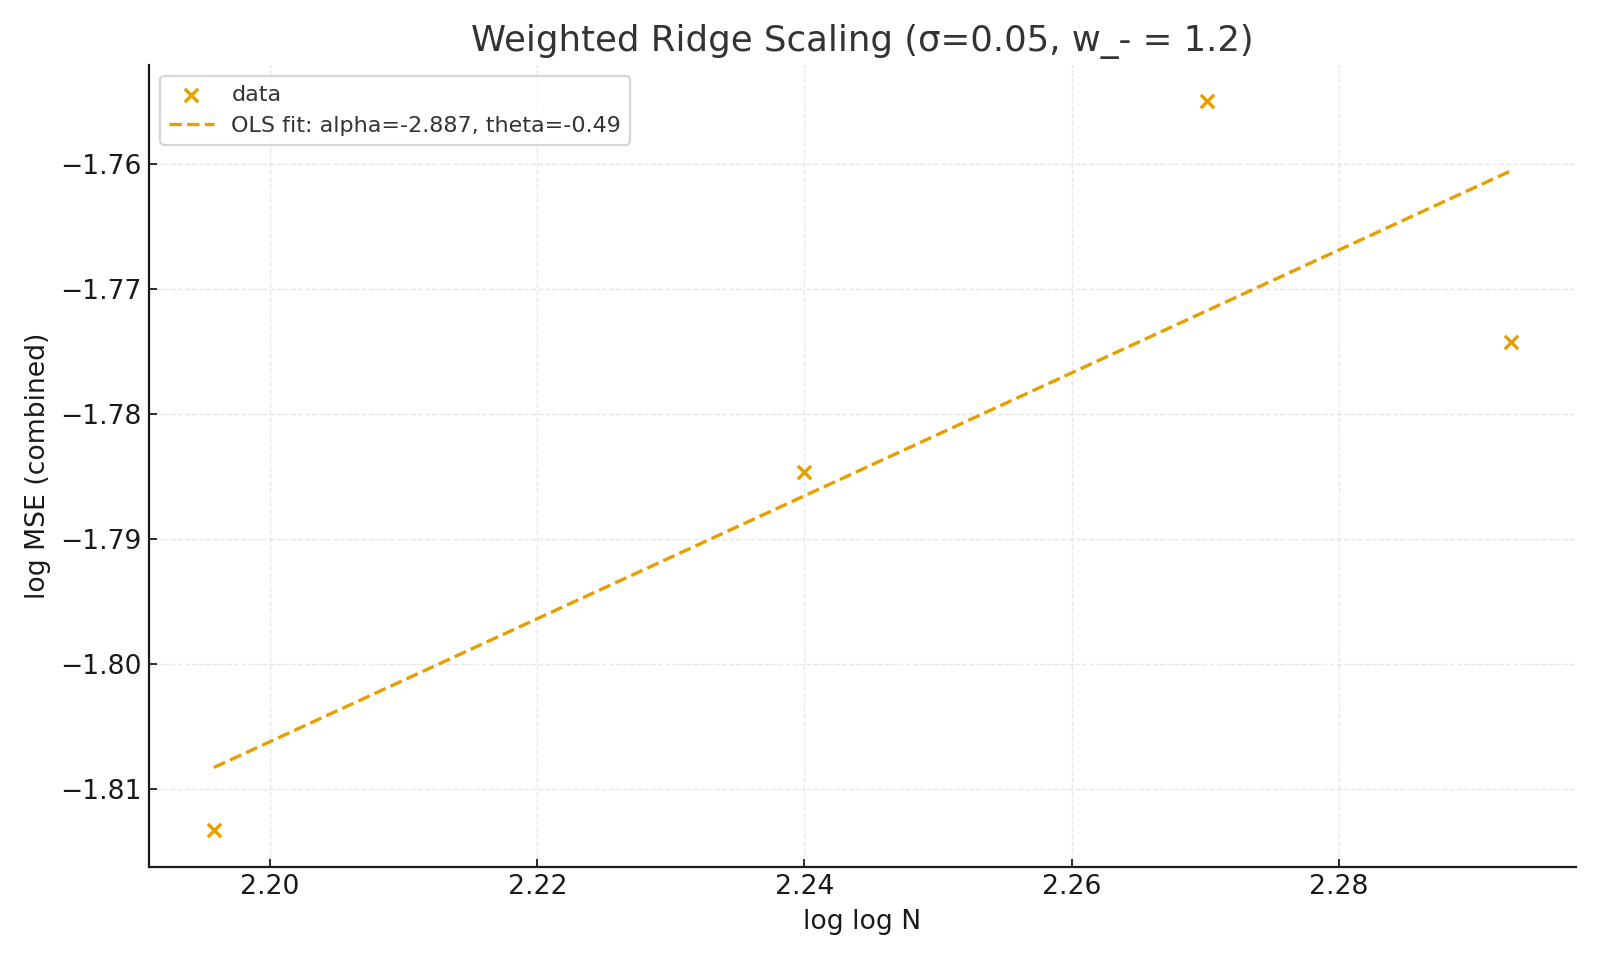
\includegraphics[width=0.78\linewidth]{figures/weighted_scaling.png}
  \caption{Weighted ridge scaling ($\sigma=0.05$, $w_-=1.2$). OLS fit on $\log(\mathrm{MSE}^*)=\alpha-\theta\log\log N$ with the displayed $(\alpha,\theta)$.}
\end{figure}

\begin{figure}[h]
  \centering
  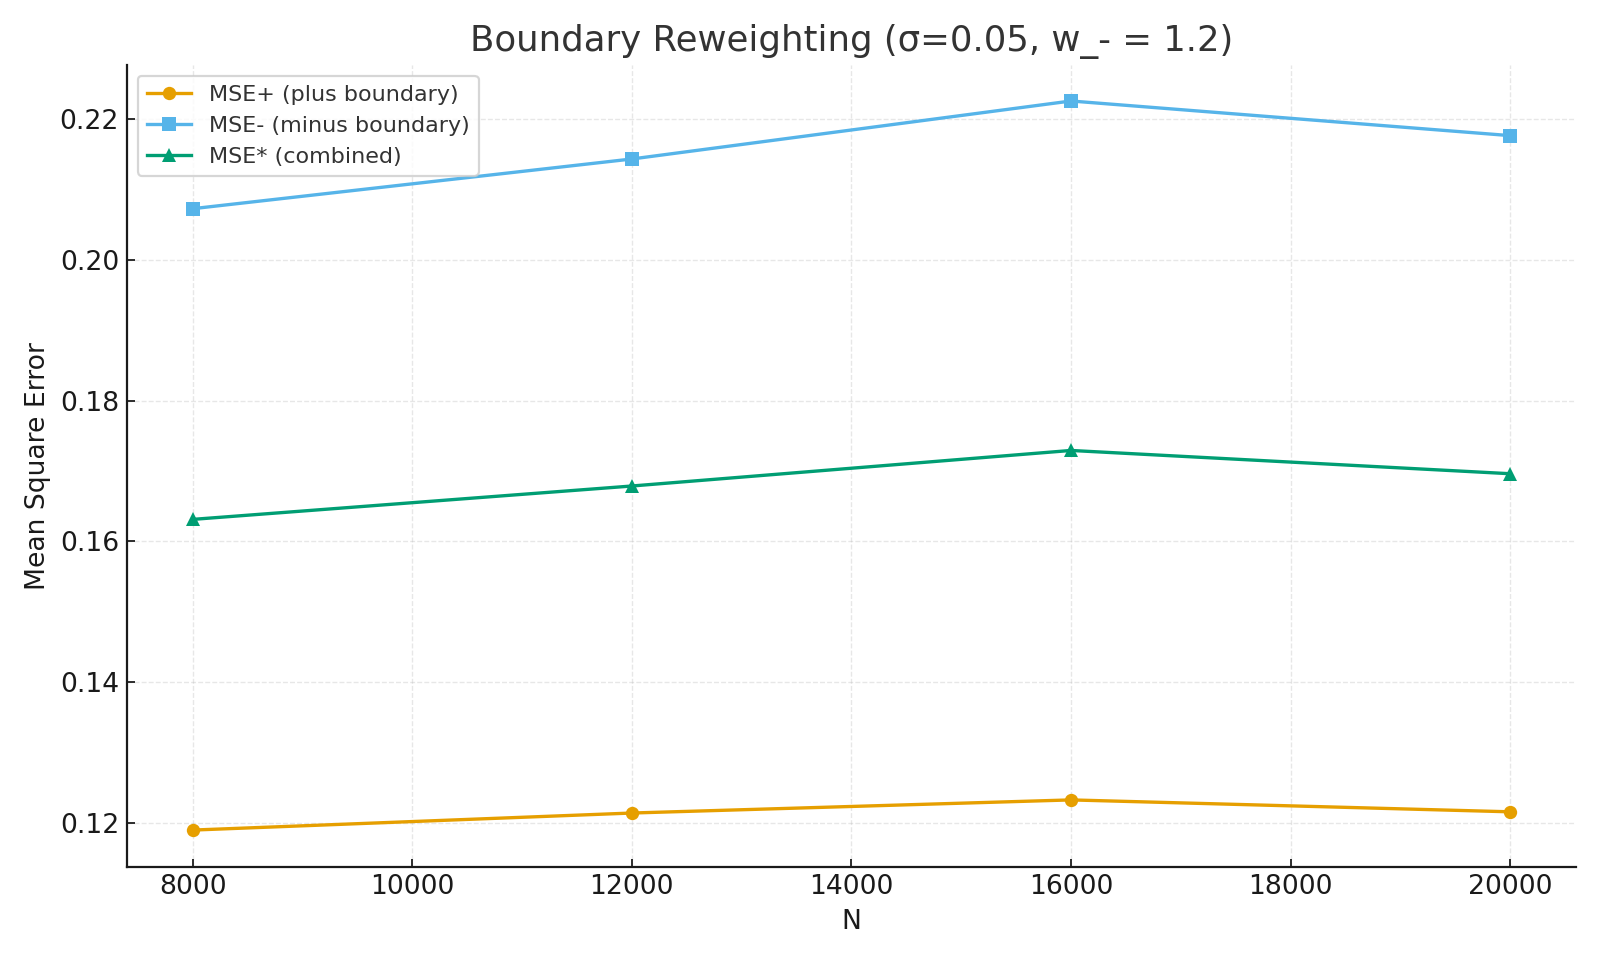
\includegraphics[width=0.78\linewidth]{figures/boundary_reweighting.png}
  \caption{Boundary-wise comparison under $w_-=1.2$: plus/minus/combined MSE.}
\end{figure}

\begin{table}[h]
\centering
\begin{tabular}{c|c|c|c}
\hline
$N$ & MSE$_+$ & MSE$_-$ & MSE$^\ast$ \\
\hline
8000  & 0.118995 & 0.207245 & 0.163120 \\
12000 & 0.121417 & 0.214303 & 0.167860 \\
16000 & 0.123280 & 0.222539 & 0.172909 \\
20000 & 0.121589 & 0.217620 & 0.169604 \\
\hline
\end{tabular}
\caption{Summary of boundary-wise and combined errors for $\sigma=0.05$, $w_-=1.2$.}
\end{table}

\section{Conclusion}
These results support stability of the NB/BD approximation under boundary reweighting. This is not a proof of RH.

\begin{thebibliography}{9}
\bibitem{baezduarte2003} L.~B\'aez--Duarte, \emph{A strengthening of the Nyman--Beurling criterion}, Rend.\ Lincei \textbf{14} (2003), 5--11.
\bibitem{conrey2003} J.~B.\ Conrey, \emph{The Riemann Hypothesis}, Notices AMS \textbf{50} (2003), 341--353.
\bibitem{titchmarsh1986} E.~C.\ Titchmarsh, \emph{The Theory of the Riemann Zeta-Function}, 2nd ed., OUP, 1986.
\end{thebibliography}

\end{document}
